% Proyek 07 -- Finding the Best Acoustic Features
% IEEE conference mini-paper (6-8 pages). Integration: Member C.
% Sources of every section are listed in paper/README.md. Text marked \TODO{...} must be
% completed or confirmed by the team before submission; remove the \TODO macro at the end.
\documentclass[conference]{IEEEtran}
\IEEEoverridecommandlockouts

\usepackage{cite}
\usepackage{amsmath,amssymb}
\usepackage{graphicx}
\usepackage{booktabs}
\usepackage{xcolor}
\usepackage{url}

% Figures live in the repository folders; keep these paths when compiling from paper/.
\graphicspath{{../figures/}{../progres_anggota_b/figures/sa_en/}}

\newcommand{\TODO}[1]{\textcolor{red}{[TODO: #1]}}

\begin{document}

\title{Finding the Best Acoustic Features: Simulated Annealing\\
Feature Selection for Speaker-Independent Speech Emotion Recognition}

\author{
\IEEEauthorblockN{\TODO{Member A name}}
\IEEEauthorblockA{\TODO{Affiliation}}
\and
\IEEEauthorblockN{\TODO{Member B name}}
\IEEEauthorblockA{\TODO{Affiliation}}
\and
\IEEEauthorblockN{\TODO{Member C name}}
\IEEEauthorblockA{\TODO{Affiliation}}
}

\maketitle

% ---------------------------------------------------------------------------
\begin{abstract}
Speech emotion recognition systems often rely on large sets of acoustic features, yet it is
unclear which features are needed. We ask whether a feature subset found by simulated
annealing (SA) can match the full feature set, and whether that subset is stable across
speakers. Using the speech part of RAVDESS (24 actors, 8 emotions) with a strictly
speaker-independent split, we extract 90 utterance-level acoustic features and search for a
subset with an SA wrapper whose objective is cross-validated macro F1 on the training speakers
minus a size penalty. On four unseen test speakers, evaluated once, an SVM on the 52 selected
features reaches a macro F1 of 0.469 [95\% CI 0.407, 0.523], indistinguishable from the same
SVM on all 90 features (0.469; paired difference +0.001 [$-$0.045, +0.052]). The subset is not
more fragile under additive noise, and subsets selected on different speaker partitions
transfer to other partitions as well as on their own. However, the selected features themselves
are unstable (Nogueira stability 0.11), only slightly above random subsets of the same size,
which we attribute to redundant, interchangeable features. Sad is the hardest emotion; listening
checks show that most of its errors come from speaker-specific delivery that utterance-level
statistics do not capture.
\end{abstract}

\begin{IEEEkeywords}
speech emotion recognition, feature selection, simulated annealing, selection stability,
speaker-independent evaluation, robustness
\end{IEEEkeywords}

% ---------------------------------------------------------------------------
\section{Introduction}

Speech emotion recognition (SER) usually summarizes each recording as a vector of acoustic
features and classifies it \cite{akcay2020,elayadi2011}. Feature sets keep growing, although
which features carry emotional information remains unclear \cite{elayadi2011}. Compact sets such
as GeMAPS were chosen by experts \cite{eyben2016gemaps}. We instead let a search algorithm choose
a subset automatically and then test whether that choice holds up.

Our research question is: \emph{can an acoustic feature subset selected by simulated annealing
match the performance of all features, and is the subset stable across speakers?} We answer it
under conditions designed to avoid optimistic estimates: speakers never appear in more than one
of train, validation, and test; every selection and tuning decision uses train and validation
only; and the test speakers are evaluated exactly once for all methods.

Our contributions are:
\begin{itemize}
\item an SA wrapper over 90 acoustic features with a size penalty, compared with mutual
information (MI) filtering, hill climbing, and random subsets at equal size;
\item a single, pre-registered test evaluation of 12 final models with bootstrap confidence
intervals and paired tests;
\item a failure analysis covering selection stability across five speaker partitions,
cross-partition transfer, additive noise at three signal-to-noise ratios, and listening-based
error analysis.
\end{itemize}

% ---------------------------------------------------------------------------
\section{Related Work}

\emph{Acoustic features for SER.} Surveys group SER features into prosodic (fundamental
frequency F0 and energy), spectral, such as mel-frequency cepstral coefficients (MFCC), and
voice quality features \cite{akcay2020,elayadi2011}. El Ayadi \emph{et al.} note that it is
still unclear which features discriminate emotions best, which has led many systems to use
large feature sets \cite{elayadi2011}. GeMAPS proposes a small parameter set selected from theory
and empirical evidence to make affective research comparable \cite{eyben2016gemaps}.

\emph{Feature selection.} Filter methods score features individually, whereas wrappers evaluate
subsets with the target classifier \cite{guyon2003featsel}. Wrappers capture feature
interactions but can overfit the data used to score subsets \cite{kohavi1997wrappers}. Simulated
annealing \cite{kirkpatrick1983sa} is a natural wrapper search for binary subset spaces because
it can escape local optima that trap greedy hill climbing.

\emph{Selection stability.} A subset that changes with the data is hard to interpret. Nogueira
\emph{et al.} \cite{nogueira2018stability} propose a stability index with desirable properties,
including correction for chance and support for subsets of different sizes, which we use here.

% ---------------------------------------------------------------------------
\section{Data and Features}

\subsection{Dataset}
We use the audio-only speech part of RAVDESS \cite{livingstone2018ravdess}: 1{,}440 WAV
recordings from 24 professional actors (12 female, 12 male) speaking two neutral sentences in
eight emotions (neutral, calm, happy, sad, angry, fearful, disgust, surprised). Seven emotions are
recorded at normal and strong intensity and neutral only at normal intensity, so neutral has 96
recordings and every other emotion 192. Labels are the emotions the actors were asked to portray
and are read from the file names. The dataset is licensed CC BY-NC-SA 4.0.

\subsection{Preprocessing}
Each recording is converted to mono, resampled from 48 to 16~kHz, and trimmed of leading and
trailing silence with a 30~dB threshold below the peak, using librosa \cite{mcfee2015librosa}.
Loudness differs between actors by up to 18.5~dB, so we extracted features with and without peak
normalization and chose on validation: peak normalization improved the 90-feature SVM from 0.485
to 0.517 macro F1 (Random Forest: 0.432 to 0.464) and was used for all later experiments.

\subsection{Features}
Each recording is summarized by 90 utterance-level features (Table~\ref{tab:features}). Frame
features use a 32~ms window and 10~ms hop and are summarized by mean and standard deviation. MFCCs
\cite{davis1980mfcc} exclude the 0th coefficient. F0 is estimated with pYIN \cite{mauch2014pyin}
between 65 and 500~Hz and summarized by robust percentiles. Five recordings without voiced frames
receive F0 statistics of 0 and a voiced ratio of 0. All feature tables can be regenerated from the
audio with one script, bit for bit.

\begin{table}[t]
\caption{The 90 acoustic features}
\label{tab:features}
\centering
\small
\begin{tabular}{@{}lrl@{}}
\toprule
Group & $n$ & Features \\
\midrule
MFCC & 26 & MFCC 1--13, mean and std \\
Delta MFCC & 26 & $\Delta$MFCC 1--13, mean and std \\
Prosody & 6 & F0 mean, std, P5, P95, range; voiced ratio \\
Energy & 3 & RMS mean, std, max \\
ZCR & 2 & mean, std \\
Spectral & 8 & centroid, bandwidth, rolloff, flatness; mean, std \\
Contrast & 7 & spectral contrast, 7 bands, mean \\
Chroma & 12 & 12 pitch classes, mean \\
\midrule
Total & 90 & \\
\bottomrule
\end{tabular}
\end{table}

On the training speakers, 39 of 4{,}005 feature pairs correlate with $|r|>0.8$, forming 17
groups of redundant features, for example the three energy features ($r=0.96$--$0.99$) and ZCR,
spectral centroid, and rolloff. We use these groups when measuring stability.

% ---------------------------------------------------------------------------
\section{Method}

\subsection{Classifier and baseline}
Standardization and classification are wrapped in one scikit-learn pipeline
\cite{pedregosa2011sklearn}, so scaling statistics are fitted on training folds only. Because
neutral has half as many recordings, classifiers use balanced class weights and are tuned for
macro F1 with 4-fold speaker-grouped cross-validation (CV) on the 16 training actors. The baselines
are an RBF SVM ($C=1$, $\gamma=0.005$) and a Random Forest (400 trees) on all 90 features.

\subsection{Simulated annealing feature selection}
A subset is a binary vector $s\in\{0,1\}^{90}$ with $|s|\ge5$. SA maximizes
\begin{equation}
J(s) = \mathrm{F1}_{\mathrm{CV}}(s) - \lambda\,\frac{|s|}{90},
\label{eq:objective}
\end{equation}
where $\mathrm{F1}_{\mathrm{CV}}$ is the 4-fold speaker-grouped CV macro F1 of an RBF SVM
($C=1$, $\gamma=$ scale) on the training actors, and $\lambda$ penalizes subset size. SA runs for
500 iterations with geometric cooling from $T_0=0.015$ to $2\times10^{-4}$, neighborhood moves of
one to three bit flips at high temperature and single flips or swaps at low temperature,
Metropolis acceptance, and up to two reheats after 80 non-improving steps. After SA, the SVM is
re-tuned on the selected subset with the same CV. We swept
$\lambda\in\{0, 0.005, 0.015, 0.03, 0.05, 0.08\}$ and chose $\lambda=0.015$, which gave the
highest validation macro F1 (Fig.~\ref{fig:lambda}); $\lambda=0.005$ selects the same 52
features.

\begin{figure}[t]
\centering
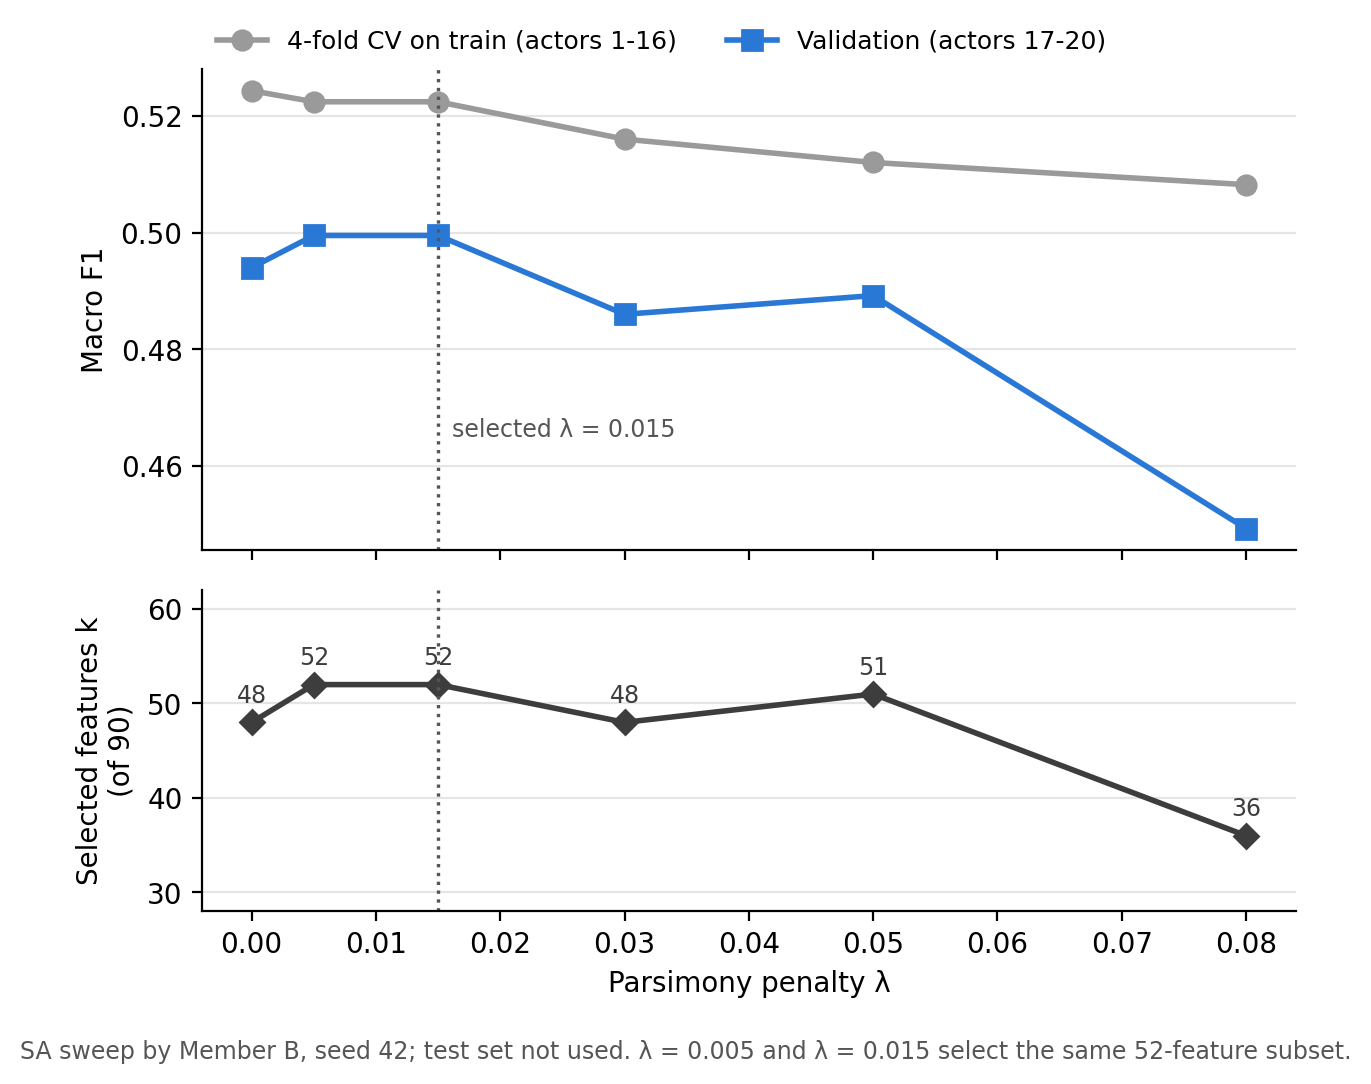
\includegraphics[width=\columnwidth]{lambda/lambda_tradeoff_en.png}
\caption{Effect of the size penalty $\lambda$ on CV and validation macro F1 (top) and on the
number of selected features (bottom). Train and validation speakers only.}
\label{fig:lambda}
\end{figure}

\subsection{Comparators}
At the same subset size we compare SA with (i) the top 52 features by mutual information computed
on training data with a $k$-nearest-neighbor estimator \cite{kraskov2004mi,ross2014mi}, with the
SVM tuned on train (which selected a linear kernel, $C=0.05$); (ii) hill climbing with the same
objective and budget (48 features); and (iii) 30 random 52-feature subsets, of which we keep the
median one by training CV. We also report Random Forest and an SVM+RF soft-voting ensemble on
both feature sets, and a two-layer MLP on all 90, the SA, and the MI features. Random Forest on
the SA subset reuses the 90-feature hyperparameters for a controlled comparison.

\subsection{Final models}
After all choices were fixed on validation, the 12 final models were refitted on train and
validation together (actors 1--20, 1{,}200 recordings).

% ---------------------------------------------------------------------------
\section{Experimental Protocol}

\emph{Speaker-independent split.} Actors 1--16 are used for training (960 recordings), 17--20
for validation (240), and 21--24 for testing (240); each part is gender-balanced and contains all
emotions. Splitting by file would leak speaker identity, because each actor repeats the same
sentences.

\emph{Stability partitions.} For stability, actors form five groups of four (two female, two
male). In partition P$k$, group $k$ is the test group, the next group is validation, and the
remaining 16 actors are training; P0 equals the main split. SA was run three times (seeds 42,
123, 2026) on each partition, giving 15 subsets. The mean Jaccard overlap of training actors
between partitions is 0.47, which bounds how similar subsets can be expected to be.

\emph{Noisy test sets.} Test recordings were mixed with white Gaussian noise or with
environmental noise from ESC-50 \cite{piczak2015esc} (rain, wind, vacuum cleaner, washing
machine, engine, keyboard typing) at 20, 10, and 0~dB SNR relative to speech power, after
preprocessing and before feature extraction. Models were trained on clean data only.

\emph{Anti-leakage rules.} A scripted audit checked that speakers do not overlap, that all
scalers are fitted inside training folds, that no model or selection code reads test data, and
that MI is computed on training data only; it reported no failures. Partitions P1--P4 contain the
test actors; their SA runs were therefore not used for any decision, and the transfer matrix
(Section~\ref{sec:failure}) was computed only after the test results were recorded. The list of
12 methods was agreed by the team before the test set was opened. Clean test and noisy test
evaluations were each run once by a script that refuses a second run.

\emph{Metrics and statistics.} We report macro F1 (primary), accuracy, and unweighted average
recall (UAR). Confidence intervals are 95\% percentile bootstrap intervals over files (1{,}000
resamples) \cite{efron1993bootstrap}. Differences between two models use a paired bootstrap on
the same resamples and an exact McNemar test on correctness \cite{dietterich1998tests}. Because
files from the same speaker are not independent and there are only four test speakers, these
intervals are likely too narrow, and we do not correct for multiple comparisons; we therefore
read a confidence interval that includes zero as ``no detectable difference'' rather than as
equivalence.

% ---------------------------------------------------------------------------
\section{Results}

\subsection{Validation}
On validation (Table~\ref{tab:val}), SA kept 52 of 90 features. It raised training CV macro F1
from 0.490 to 0.522 but lowered validation macro F1 from 0.517 to 0.500, a pattern consistent with
wrapper overfitting to the training speakers \cite{kohavi1997wrappers}. At 52 features SA scored
above the MI filter (0.426) and the random subsets (0.474 $\pm$ 0.027 over 30 subsets), and close
to hill climbing (0.503 with 48 features).

\begin{table}[t]
\caption{Validation macro F1 (actors 17--20), models trained on actors 1--16}
\label{tab:val}
\centering
\small
\setlength{\tabcolsep}{4pt}
\begin{tabular}{@{}lrrr@{}}
\toprule
Method & $k$ & CV F1 (train) & Val F1 \\
\midrule
SVM, all features & 90 & 0.490 & 0.517 \\
SVM, SA (seed 42) & 52 & 0.522 & 0.500 \\
SVM, SA (3 seeds, mean $\pm$ SD) & 52.7 $\pm$ 1.2 & 0.510 $\pm$ 0.011 & 0.497 $\pm$ 0.013 \\
SVM, MI top-52 & 52 & 0.472 & 0.426 \\
SVM, hill climbing & 48 & 0.512 & 0.503 \\
SVM, random (30 subsets) & 52 & 0.428 $\pm$ 0.020 & 0.474 $\pm$ 0.027 \\
RF, all features & 90 & 0.442 & 0.464 \\
RF, SA & 52 & -- & 0.452 \\
SVM+RF, all features & 90 & 0.464 & 0.524 \\
SVM+RF, SA & 52 & 0.489 & 0.506 \\
\bottomrule
\end{tabular}
\end{table}

\subsection{Test (single evaluation)}
Table~\ref{tab:test} lists the test results of all 12 final models and Table~\ref{tab:paired}
the planned paired comparisons. The main comparison answers the research question: the SVM on the
52 SA features is indistinguishable from the SVM on all 90 features (0.469 vs.\ 0.469; difference
+0.001 [$-$0.045, +0.052], McNemar $p=1.00$). The same holds for Random Forest and the ensemble.
SA tends to score above MI (+0.047) and random subsets (+0.035), but both intervals include zero.

The ranking of model families changed from validation to test: SVM was best on validation, while
Random Forest was best on test (0.513). The MLP on SA features scored highest overall (0.554) and
is the only comparison whose interval excludes zero, but it is a single-seed model, its validation
score with the same seed was lower than the 90-feature MLP (0.447 vs.\ 0.493), its five-seed
validation means were equal (0.477 vs.\ 0.477), and $p=0.018$ would not survive a Bonferroni
correction for seven comparisons. We therefore do not treat it as evidence that SA features help
MLPs.

\begin{table}[t]
\caption{Test results (actors 21--24, $n=240$), evaluated once}
\label{tab:test}
\centering
\small
\setlength{\tabcolsep}{3.5pt}
\begin{tabular}{@{}lrrrr@{}}
\toprule
Method & $k$ & Acc. & Macro F1 [95\% CI] & UAR \\
\midrule
SVM, all & 90 & 0.488 & 0.469 [0.412, 0.524] & 0.504 \\
SVM, SA & 52 & 0.483 & 0.469 [0.407, 0.523] & 0.496 \\
SVM, MI & 52 & 0.433 & 0.422 [0.360, 0.480] & 0.449 \\
SVM, HC & 48 & 0.488 & 0.473 [0.415, 0.528] & 0.500 \\
SVM, random & 52 & 0.454 & 0.435 [0.380, 0.485] & 0.473 \\
RF, all & 90 & 0.529 & 0.513 [0.448, 0.569] & 0.535 \\
RF, SA & 52 & 0.525 & 0.503 [0.440, 0.563] & 0.520 \\
SVM+RF, all & 90 & 0.513 & 0.497 [0.436, 0.553] & 0.516 \\
SVM+RF, SA & 52 & 0.492 & 0.480 [0.417, 0.534] & 0.496 \\
MLP, all & 90 & 0.488 & 0.483 [0.415, 0.544] & 0.500 \\
MLP, SA & 52 & 0.567 & 0.554 [0.487, 0.609] & 0.570 \\
MLP, MI & 52 & 0.508 & 0.502 [0.435, 0.559] & 0.520 \\
\bottomrule
\end{tabular}
\end{table}

\begin{table}[t]
\caption{Paired test comparisons (macro F1 difference A $-$ B)}
\label{tab:paired}
\centering
\small
\begin{tabular}{@{}lrr@{}}
\toprule
A $-$ B & Difference [95\% CI] & McNemar $p$ \\
\midrule
SVM: SA $-$ all & +0.001 [$-$0.045, +0.052] & 1.000 \\
SVM: SA $-$ MI & +0.047 [$-$0.013, +0.112] & 0.155 \\
SVM: SA $-$ HC & $-$0.004 [$-$0.053, +0.044] & 1.000 \\
SVM: SA $-$ random & +0.035 [$-$0.015, +0.083] & 0.337 \\
RF: SA $-$ all & $-$0.010 [$-$0.058, +0.036] & 1.000 \\
SVM+RF: SA $-$ all & $-$0.017 [$-$0.066, +0.028] & 0.500 \\
MLP: SA $-$ all & +0.071 [+0.014, +0.130] & 0.018 \\
\bottomrule
\end{tabular}
\end{table}

\begin{figure}[t]
\centering
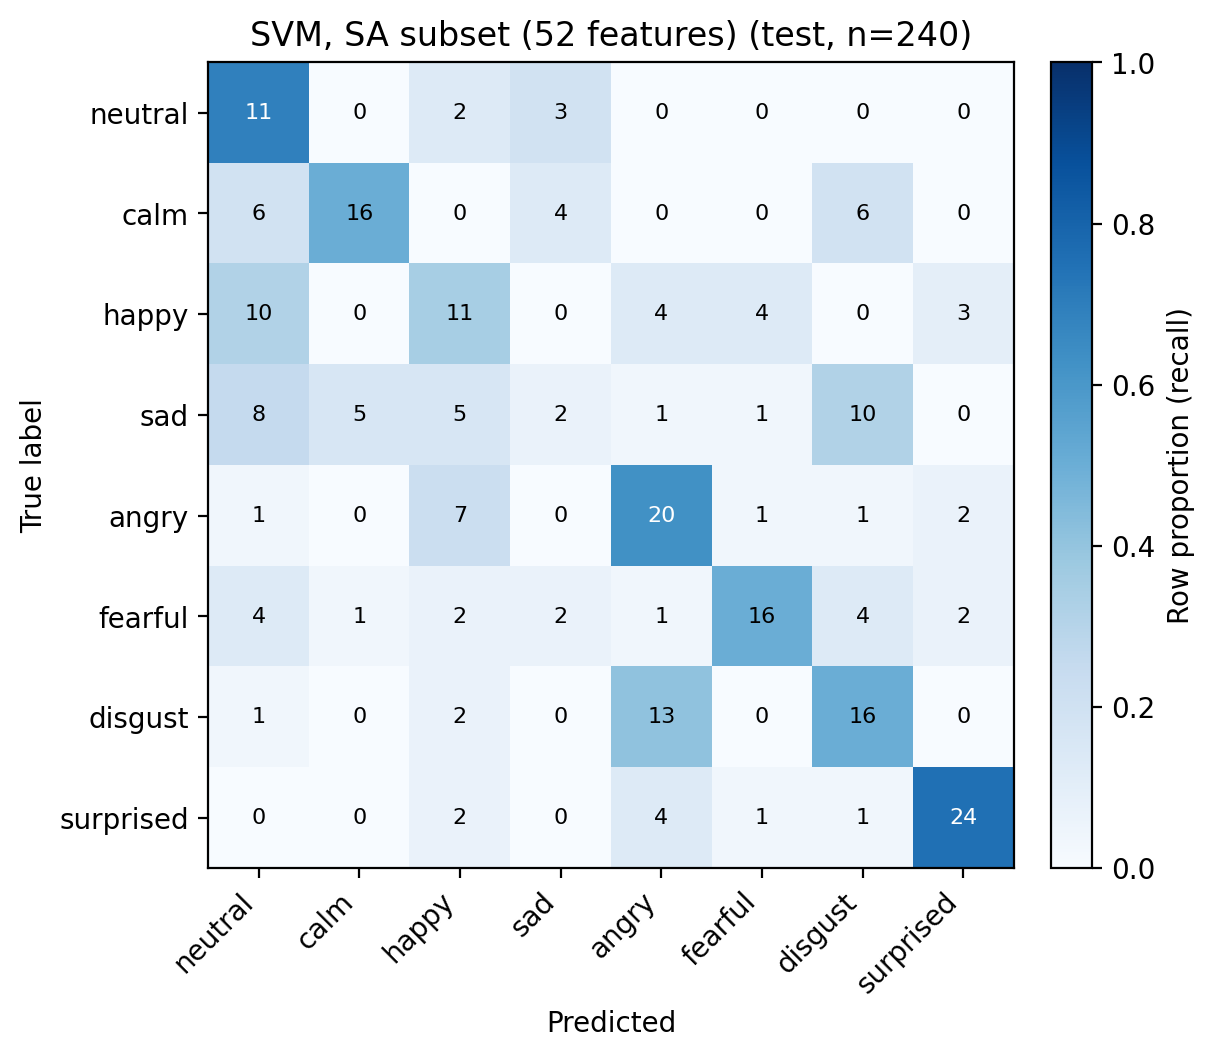
\includegraphics[width=0.9\columnwidth]{test_eval/cm_SVM_SA52_en.png}
\caption{Test confusion matrix of the SVM on the 52 SA features. Colors show recall per true
class; numbers are file counts.}
\label{fig:cm}
\end{figure}

% ---------------------------------------------------------------------------
\section{Failure Analysis}
\label{sec:failure}

\subsection{Stability of the selected subset}
Across the 15 SA runs, subset size was $46.3\pm5.8$ (38--58). The Nogueira stability index was
0.106 over all runs and 0.153 within a partition. Mean pairwise Jaccard similarity was 0.395,
only slightly above 0.344 for random subsets of the same sizes; at the level of redundant groups
it was 0.489 vs.\ 0.437. Only the voiced ratio was selected in all 15 runs. The subset that SA
returns is therefore not a stable ``best'' set.

The transfer matrix (Fig.~\ref{fig:transfer}) shows why this does not hurt accuracy. A subset
selected on partition $i$ was retrained and evaluated on each partition $j$. Subsets scored 0.473
on their own partition and 0.484 on other partitions, and all 90 features scored 0.489. Subsets
thus do not overfit their speakers, and different subsets perform alike. Scores varied more
between evaluation partitions (0.463--0.502) than between subsets (0.476--0.486): which speakers
are tested matters more than which subset is used. Together with the redundancy groups, this
suggests that many features are interchangeable and SA picks one of many equally good
combinations.

\begin{figure}[t]
\centering
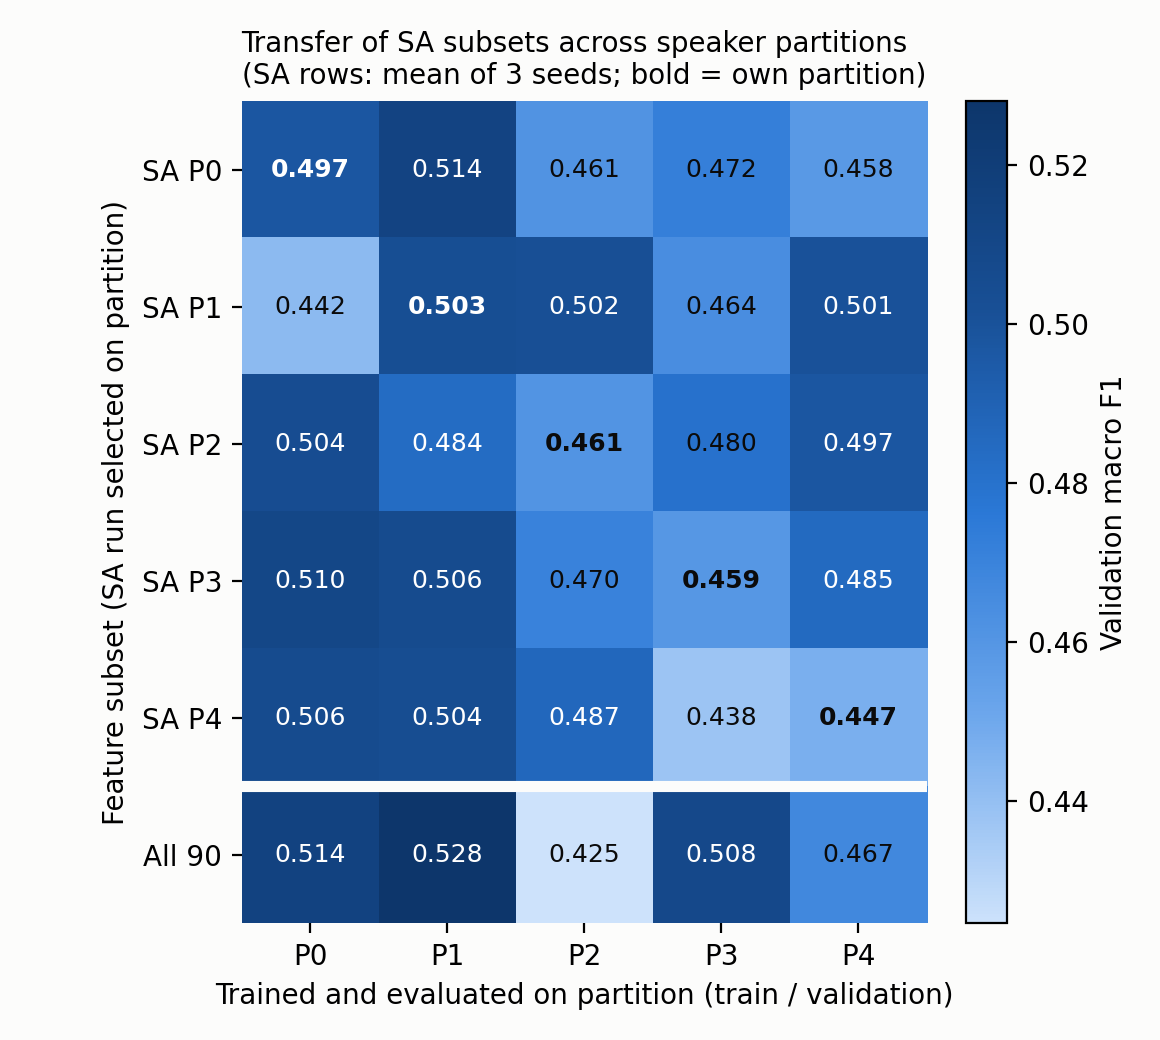
\includegraphics[width=0.9\columnwidth]{stability/stab_03_transfer.png}
\caption{Transfer of SA subsets across speaker partitions (validation macro F1, mean of three
seeds). Bold cells: subset evaluated on the partition it was selected on. Last row: all 90
features. Computed after the test results were recorded.}
\label{fig:transfer}
\end{figure}

\subsection{Robustness to additive noise}
Fig.~\ref{fig:noise} shows test macro F1 under noise. Environmental noise degrades the SVM
gradually (0.469, 0.441, 0.310, 0.146 from clean to 0~dB). White noise collapses the RBF SVMs
already at 20~dB: every file is predicted as fearful (macro F1 0.029). This matches the measured
feature shift: at 20~dB white noise, spectral and contrast features move by 3.9 and 3.0 training
standard deviations on average, far outside the training distribution of an RBF kernel. Random
Forest degrades more gently (0.173 at 20~dB). The SA subset was never more fragile than all
features (largest difference 0.004), so the hypothesis that a subset rich in spectral features
would degrade fastest is not supported. The MI subset appears more robust to white noise
(0.068--0.106), but its SVM uses a linear kernel, so this effect cannot be attributed to the
features.

\begin{figure}[t]
\centering
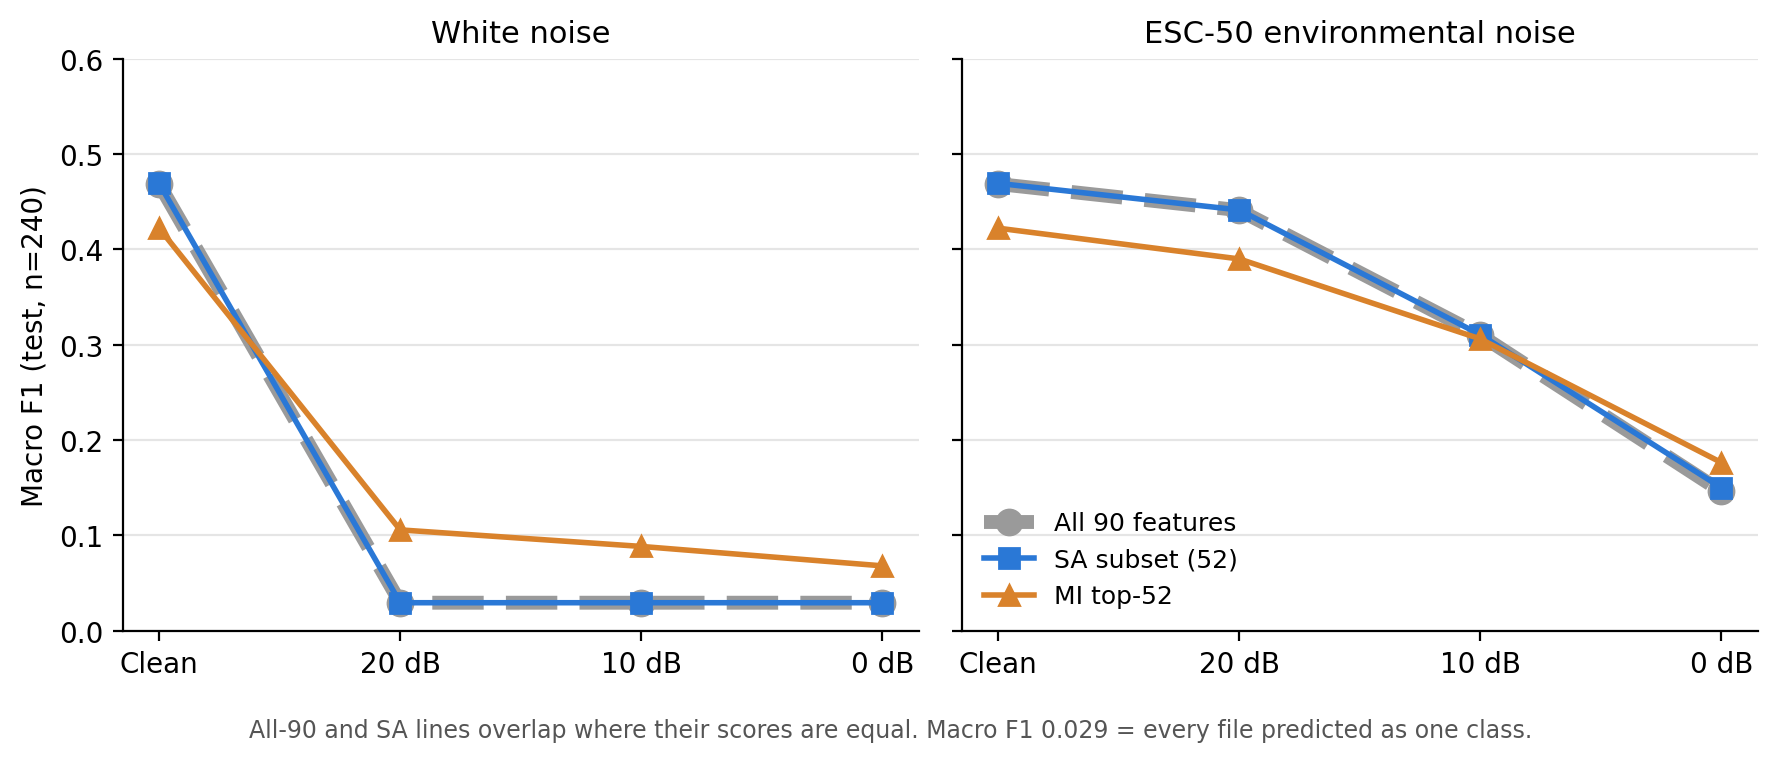
\includegraphics[width=\columnwidth]{test_eval/noise_macro_f1_svm_en.png}
\caption{Test macro F1 of the SVM under white and ESC-50 noise. Models were trained on clean
data. The all-feature and SA lines overlap where their scores are equal.}
\label{fig:noise}
\end{figure}

\subsection{Error analysis}
Sad is the hardest emotion: on average 10.7 of 12 models misclassify a sad file, and 17 of 32 sad
files are misclassified by all models, mostly as disgust or neutral. Disgust is often predicted as
angry. Normal intensity is harder than strong intensity (SVM-SA accuracy 0.43 vs.\ 0.55), while
female and male speakers do not differ (0.48). The all-feature and SA SVMs fail on the same files
with the same labels (87 of 105 jointly wrong files), so the errors are not caused by feature
selection.

We inspected four files that all models got wrong and listened to them. Three sad files clearly
sound sad to a listener: one is drawn out with long pauses, one is close to neutral, and one
sounds as if the speaker is about to cry. In the acoustic inspection, the near-neutral file has
the same F0 contour and median (182~Hz) as the actor's neutral recording of the same sentence; the
drawn-out file contains a long, noisy unvoiced segment that raises its zero-crossing features
toward disgust; and in the crying file pitch tracking finds voicing in only 26\% of frames. Speaking rate, pause
duration, and crying voice are not captured by our utterance-level statistics; only the voiced
ratio comes close. The fourth file, labeled disgust, sounds angry because of strong emphasis, as
all models predicted, suggesting ambiguity in the acted labels. These judgments come from one
listener who knew the labels and are qualitative.

% ---------------------------------------------------------------------------
\section{Discussion and Limitations}

\emph{Fewer features, same accuracy.} With 58\% of the features, the SA subset performed like the
full set on unseen speakers with SVM, Random Forest, and the ensemble on clean test data, and with
the SVM under all six noise conditions.
Feature selection therefore bought a smaller model, not a more accurate one. The validation
results already hinted at this: SA increased training CV macro F1 but not validation macro F1,
the typical sign of a wrapper adapting to the speakers it is scored on
\cite{kohavi1997wrappers}. A size penalty and speaker-grouped CV limited, but did not remove,
this effect. That SA scored above MI and random subsets of the same size on validation, but not
detectably on test, shows how much a four-speaker evaluation can move such differences.

\emph{An unstable subset is not a wrong subset.} The low stability index would suggest that SA
found nothing reliable. The transfer matrix and the redundancy groups suggest a different reading:
the feature space contains many interchangeable features, and SA returns one of many equally good
combinations. The individual features in a single SA subset should therefore not be interpreted
as ``the'' emotion features. Statements are safer at the level of feature groups and of features
that are selected almost always, such as the voiced ratio (15 of 15 runs) and the standard
deviations of low-order MFCCs and their deltas (14 of 15 runs). This also clarifies how automatic
selection relates to expert sets such as GeMAPS \cite{eyben2016gemaps}: when features are
redundant, a search can match an expert set's size and accuracy without converging to a unique
set, so expert knowledge remains useful for choosing among equivalent subsets.

\emph{What limits performance.} Neither the test errors nor the noise failures came from the
selection step. Scores varied more across speaker groups than across subsets, sad was confused with neutral
in speaker-specific ways, and white noise broke the RBF SVM through a distribution shift in
spectral features that affected all feature sets alike. Improvements are more likely to come from
speaker normalization, features of rhythm and voice quality, and noise-aware training than from a
better subset search over the same 90 features.

Limitations. (1) The test set has only four speakers, and file-level bootstrap intervals are
likely too narrow. (2) SA on the main split used three seeds, and hill climbing and the $\lambda$
sweep one seed each, instead of the planned five, three, and three. (3) The stability runs on
P1--P4 were performed before the main results were final and include the test actors; their
validation scores were not used for any decision. (4) RAVDESS contains acted speech from
North American English speakers reading two sentences, so results may not hold for spontaneous
speech. (5) Models were trained on clean audio only; no noise augmentation was used. (6) The
error analysis covers four files and one listener.

% ---------------------------------------------------------------------------
\section{Conclusion}

An SA wrapper reduced 90 acoustic features to 52 without a detectable loss in speaker-independent
test performance and without additional sensitivity to noise. The selected subset, however, is
not a stable answer to ``which features are best'': different runs pick different but
interchangeable features. Future work should add rhythm features (speaking rate and pauses),
voice quality features such as jitter, shimmer, and HNR, and per-speaker normalization, which
our error analysis suggests address the remaining failures, and evaluate on more speakers.

\section*{Author Contributions}
\TODO{Confirm.} Member A prepared the dataset, preprocessing, features, splits, noisy test sets,
redundancy analysis, the MI comparator, and the MLP experiment. Member B implemented the
baselines, SA, hill climbing, random subsets, ensembles, the $\lambda$ sweep, and the final
models. Member C built the evaluation module and anti-leakage audit, ran the single test and noise
evaluations, the stability and transfer analyses, the error analysis, and the demo, and integrated
the paper.

\section*{Code and Data Availability}
\TODO{Repository URL and access.} All numbers in this paper are produced by the scripts in the
project repository from \texttt{results/main\_table.csv}, \texttt{results/test\_eval/},
\texttt{results/noise\_eval/}, and \texttt{results/stability\_*}.

\bibliographystyle{IEEEtran}
\bibliography{references}

\end{document}
